\newpage
\section{RESULTADOS}
Os modelos gerados pelo código fonte LaTeX estão disponíveis em um repositório do GitHub. Para realizar o download acesse o link:\\https://github.com/RafaeleSoares/Modelos-de-documentos-em-Latex-para-o-iftm-ituiutaba\\

Clique em "Clone or Download".
\begin{figure}[h]
	\centering
	
\includegraphics[scale=0.5]{imagens/git/git1.png}\\
	\caption{Como realizar o download dos modelos. Passo1.}
	\label{git1}
\end{figure}

Clique em "Download ZIP".
\begin{figure}[h]
	\centering
	
\includegraphics[scale=0.5]{imagens/git/git2.png}\\
	\caption{Como realizar o download dos modelos. Passo2.}
	\label{git2}
\end{figure}

Após realizar o download dos modelos, e se o LaTeX já estiver pronto para o uso, o estudante será capaz de começar a escrever seu documento.

A seguir serão mostrados os resultados dos modelos dos trabalhos acadêmicos do IFTM Ituiutaba.

\subsection{RESULTADO DO MODELO DE RELATÓRIO DE ESTÁGIO}
O modelo do relatório de estágio foi feito seguindo as normas para elaboração de relatório de estágio \cite{manualEstagio}.

\newpage
A capa do relatório (Figura \ref{capaest}) gerada com o LaTeX e o modelo desenvolvido contém todos os elementos que constam no regulamento.\\

\begin{figure}[h]
	\centering
	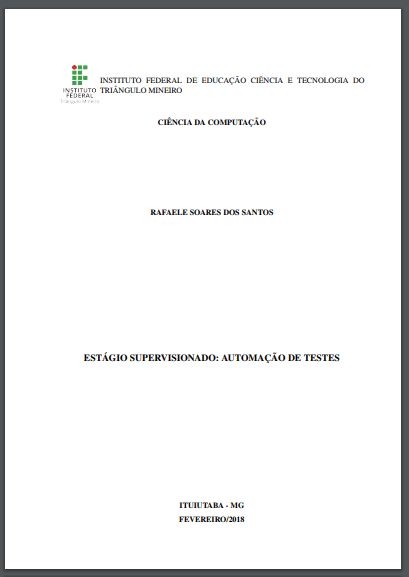
\includegraphics{imagens/relatorioEstagio/Capa.png}\\
	\caption{Exemplo da capa do relatório de estágio gerado em LaTeX.}
	\label{capaest}
\end{figure}

\newpage
A folha de rosto do relatório (Figura \ref{folharostoest}) contém todos os elementos que constam no regulamento para a identificação do trabalho.\\
\begin{figure}[h]
	\centering
	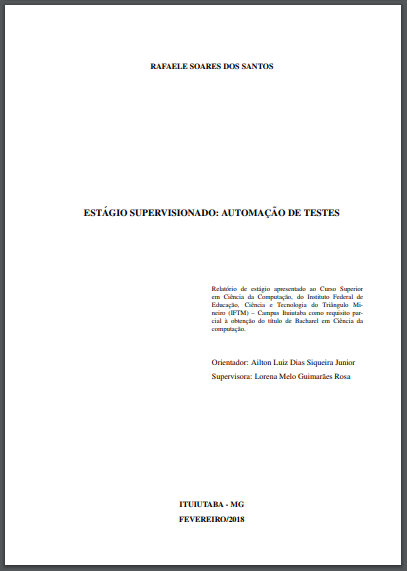
\includegraphics{imagens/relatorioEstagio/FolhaRosto.png}\\
	\caption{Exemplo da folha de rosto do relatório de estágio gerado em LaTeX.}
	\label{folharostoest}
\end{figure}

\newpage
A folha de identificação do relatório (Figura \ref{folhaidentest}) apresenta todos os elementos que constam no regulamento para a identificação do trabalho.\\
\begin{figure}[h]
	\centering
	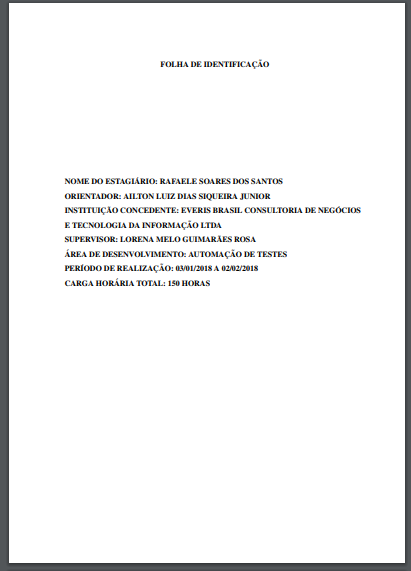
\includegraphics{imagens/relatorioEstagio/FolhaIdentif.png}\\
	\caption{Exemplo da folha de identificação do relatório de estágio gerado em LaTeX.}
	\label{folhaidentest}
\end{figure}

\newpage
A Figura \ref{dedicest} mostra um exemplo de dedicatória gerado em LaTeX para o relatório de estágio.\\
\begin{figure}[h]
	\centering
	
\includegraphics{imagens/relatorioEstagio/Dedicatoria.png}\\
	\caption{Exemplo da página de dedicatória do relatório de estágio gerado em LaTeX.}
	\label{dedicest}
\end{figure}

\newpage
A Figura \ref{agradest} mostra um exemplo de agradecimento gerado em LaTeX para o relatório de estágio.\\
\begin{figure}[h]
	\centering
	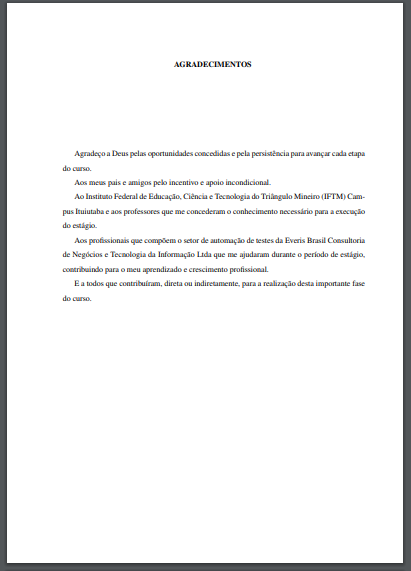
\includegraphics{imagens/relatorioEstagio/Agradecimento.png}\\
	\caption{Exemplo da página de agradecimento do relatório de estágio gerado em LaTeX.}
	\label{agradest}
\end{figure}

\newpage
A Figura \ref{sumest} ilustra o sumário gerado automaticamente pelo LaTeX para o relatório de estágio.\\
\begin{figure}[h]
	\centering
	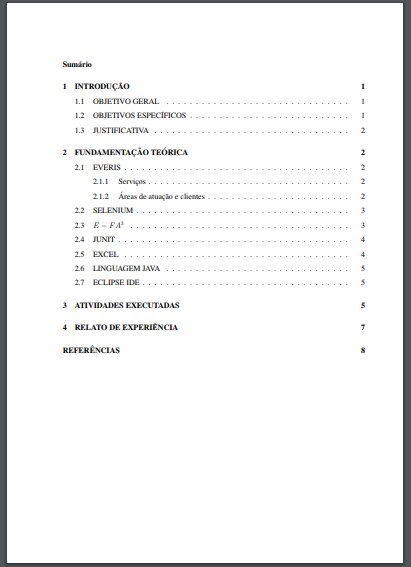
\includegraphics{imagens/relatorioEstagio/Sumario.png}\\
	\caption{Exemplo de sumario.}
	\label{sumest}
\end{figure}

\newpage
\subsection{RESULTADO DO MODELO DE PROJETO DE PESQUISA}
O modelo do projeto de pesquisa foi feito seguindo o manual para normatização de TCC \cite{manualTCC}.

A capa do projeto de pesquisa (Figura \ref{capaproj}) contém todos os elementos que constam no regulamento.\\
\begin{figure}[h]
	\centering
	\includegraphics{imagens/projetoPesq/Capa.png}\\
	\caption{Exemplo da capa do relatório do projeto de pesquisa gerado em LaTeX.}
	\label{capaproj}
\end{figure}

\newpage
A folha de rosto do projeto de pesquisa (Figura \ref{folharostoproj}) exibe todos os elementos que constam no regulamento para a identificação do trabalho.\\
\begin{figure}[h]
	\centering
	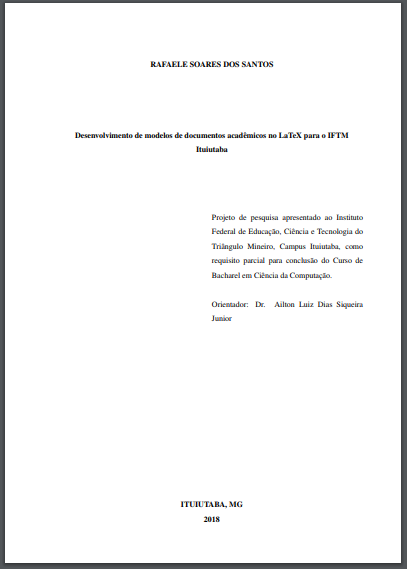
\includegraphics{imagens/projetoPesq/FolhaRosto.png}\\
	\caption{Exemplo da folha de rosto do projeto de pesquisa gerado em LaTeX.}
	\label{folharostoproj}
\end{figure}

\newpage
A Figura \ref{listafigProj} ilustra a lista de figuras gerada automaticamente pelo LaTeX para o projeto de pesquisa.\\
\begin{figure}[h]
	\centering
	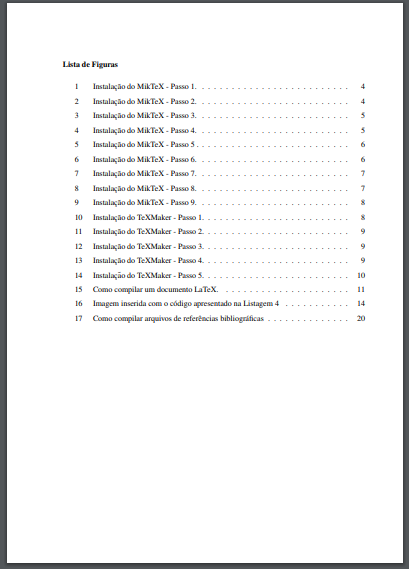
\includegraphics{imagens/projetoPesq/ListaFig.png}\\
	\caption{Exemplo de lista de figura do projeto de pesquisa gerado em LaTeX.}
	\label{listafigProj}
\end{figure}

\newpage
A Figura \ref{sumProj} ilustra o sumário gerado automaticamente pelo LaTeX para o projeto de pesquisa.\\
\begin{figure}[h]
	\centering
	\includegraphics{imagens/projetoPesq/Sumario.png}\\
	\caption{Exemplo de sumário do projeto de pesquisa gerado em LaTeX.}
	\label{sumProj}
\end{figure}

\newpage
\subsection{RESULTADO DO MODELO DE ARTIGO}
O modelo de artigo foi feito seguindo o manual para normatização de TCC\cite{manualTCC}.

A Figura \ref{iniart} ilustra a folha inicial do modelo de artigo, contendo o título, o nome do autor, o resumo, as palavras-chave, o título em língua estrangeira, o abstract e as keywords.\\
\begin{figure}[h]
	\centering
	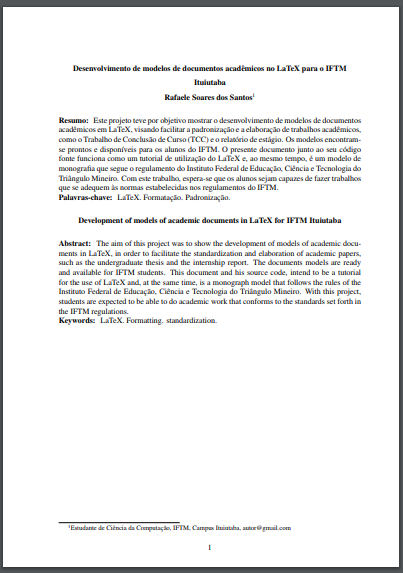
\includegraphics{imagens/artigo/folhaInicial.png}\\
	\caption{Exemplo da folha inicial do artigo gerado em LaTeX.}
	\label{iniart}
\end{figure}

\newpage
\subsection{RESULTADO DO MODELO DA MONOGRAFIA}
O modelo da monografia foi feito seguindo o manual para normatização de TCC \cite{manualTCC}.\\

A capa da monografia (Figura \ref{capamon}) contém todos os elementos que constam no regulamento.\\
\begin{figure}[h]
	\centering
	\includegraphics{imagens/monografia/Capa.png}\\
	\caption{Exemplo da capa da monografia gerado em LaTeX.}
	\label{capamon}
\end{figure}

\newpage
A folha de rosto da monografia (Figura \ref{folharostomon}) apresenta todos os elementos que constam no regulamento para a identificação do trabalho.\\
\begin{figure}[h]
	\centering
	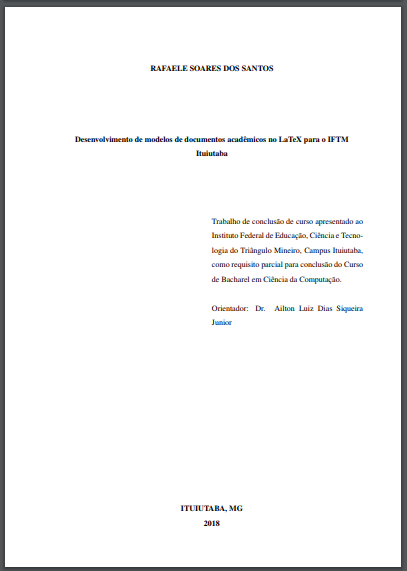
\includegraphics{imagens/monografia/FolhaRosto.png}\\
	\caption{Exemplo da folha de rosto da monografia gerado em LaTeX.}
	\label{folharostomon}
\end{figure}

\newpage
O termo de aprovação da monografia (Figura \ref{aprovmon}) exibe todos os elementos que constam no regulamento.\\
\begin{figure}[h]
	\centering
	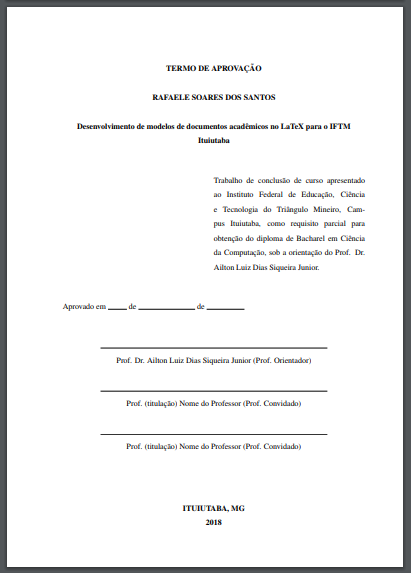
\includegraphics{imagens/monografia/TermoAprov.png}\\
	\caption{Exemplo do de termo de aprovação da monografia gerado em LaTeX.}
	\label{aprovmon}
\end{figure}

\newpage
A Figura \ref{listafigmon} ilustra a lista de figuras gerada automaticamente pelo LaTeX para a monografia.\\
\begin{figure}[h]
	\centering
	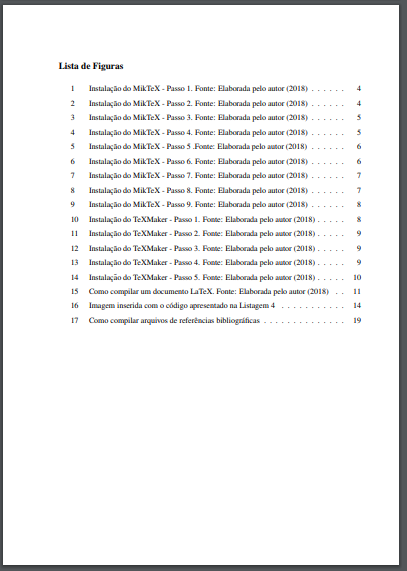
\includegraphics{imagens/monografia/ListaFig.png}\\
	\caption{Exemplo de lista de figuras do projeto de pesquisa gerado em LaTeX.}
	\label{listafigmon}
\end{figure}

\newpage
A Figura \ref{summon} ilustra o sumário gerado automaticamente pelo LaTeX para a monografia.\\
\begin{figure}[h]
	\centering
	\includegraphics{imagens/monografia/Sumario.png}\\
	\caption{Exemplo de sumário da monografia gerado em LaTeX.}
	\label{summon}
\end{figure}